\section{Results} % (fold)
\label{sec:results}
% - It would be nice to compare the performance of your reinforcement learning (RL) or Markov decision process (MDP) model to some naive baseline policies based on heuristic rules. These rules are the one you would adopt when playing yourself the game (or controlling the system).
% Then the question is "Does RL or MDP perform better than the baseline strategy ?" Experimental simulations/comparisons should be carried out in order to answer this question.

In this section, we wish to validate our model through its application on a real case problem and answer our research question detailed in section~\ref{sec:objective}.

Before jumping into the experiments themselves, let us describe the dataset we used.
We use data from a real distribution network with real generation and load profiles.

Our dataset is a slightly simplified version of the data used in Niels \textsc{Leemput} PhD thesis~\cite{Niels} which is a real urban feeder topology that was provided for the EIT-KIC InnoEnergy EVCity project~\cite{evcity} to which the second author has access for his master thesis~\cite{Quentin}.

The system is 5 nodes distribution network made of 3 households, 1 small factory considered as a flexible load and 1 transformer node of maximum power rating of $250\si{\kilo\volt}$ linking the distribution network to the medium voltage network.
All households are assumed to be connected to the same phase, with a rated neutral-to-phase voltage of $230\si{\volt}$.
In what concerns the distances, the distance between the substation node and the first connection node is $350\si{\meter}$.
Then, the distance between two successive nodes is $7.2\si{\meter}$.
A schema of the distribution network can be found in figure~\ref{fig:schema_line}.
\begin{figure}[H]
\centering
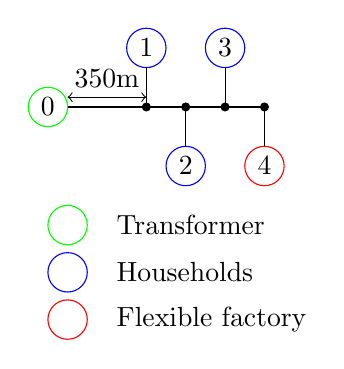
\begin{tikzpicture}[scale=0.5]
\draw (0,0) -- (5,0);
\draw [color=green] (-0.5,0) circle (0.5cm);
\node at (-0.5,0) {0};
\draw (2,0) -- (2,1);
\draw [fill=black] (2,0) circle (0.1cm);
\draw [color=blue] (2,1.5) circle (0.5cm);
\node at (2,1.5) {1};
\draw (3,0) -- (3,-1);
\draw [fill=black] (3,0) circle (0.1cm);
\draw [color=blue] (3,-1.5) circle (0.5cm);
\node at (3,-1.5) {2};
\draw (4,0) -- (4,1);
\draw [fill=black] (4,0) circle (0.1cm);
\draw [color=blue] (4,1.5) circle (0.5cm);
\node at (4,1.5) {3};
\draw (5,0) -- (5,-1);
\draw [fill=black] (5,0) circle (0.1cm);
\draw [color=red] (5,-1.5) circle (0.5cm);
\node at (5,-1.5) {4};
\draw [<->] (0, 0.25) -- (2, 0.25);
\node [above] at (1,0.25) {350m};
\draw [color=green] (0,-3) circle (0.5cm);
\node [right, xshift=0.5cm] at (0,-3) {Transformer};
\draw [color=blue] (0,-4.2) circle (0.5cm);
\node [right, xshift=0.5cm] at (0,-4.2) {Households};
\draw [color=red] (0,-5.4) circle (0.5cm);
\node [right, xshift=0.5cm] at (0,-5.4) {Flexible factory};
 \end{tikzpicture}
\caption{The real distribution network used.}
\label{fig:schema_line}
\end{figure}

The characteristics of the lines are summarized in table~\ref{tab:char_lines}.
\begin{table}[H]
  \caption{Characteristics of the line.}
  \label{tab:char_lines}
  \centering
  \begin{tabular}{c|c}
  \hline
   Impedance [$\si{\ohm\per\kilo\meter}$] & Current limit [$\si{\ampere}$] \\
   \hline
   $0.31 + \mathbf{i}0.0713$ & $210$ \\
   \hline
  \end{tabular}
\end{table}

We use real single-phase household electric power consumption profiles
that were sampled in 2008, with a 1 hour time resolution.
We also have real PV power generation profiles for all these households that are based upon measurements at an installation of the KU Leuven, also with a 1 hour resolution.
The horizon used is one week and the profiles were acquired in May.

\begin{figure}
  \begin{center}
    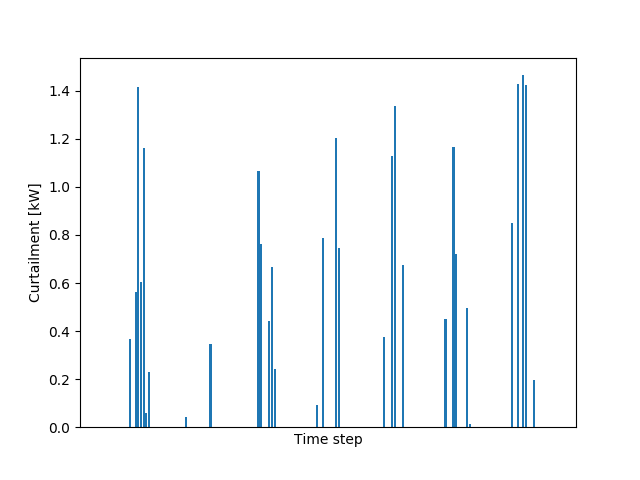
\includegraphics[scale=0.7]{./img/power_cut.png}
  \end{center}
  \caption{Power cut of house 4 following power forecast.}
  \label{fig:power_cut}
\end{figure}

Let us now present our results for the comparison between reinforcement learning based on the Markov chain model and multi-time-steps deterministic optimization.

\subsection{Assumptions}

The main assumptions of the RL decision framework are the following :
\begin{itemize}
\item We suppose that the probability distribution for load and production curtailment is discrete.
\item We suppose that the curtailment actions are discrete.
\item The flexible load is either on or off, but we can't activate the flexibility of part of the load.
\item We have to pay a large cost when voltage and current bounds are violated.
\end{itemize}

The assumptions of the optimization part are
\begin{itemize}
\item The problem is deterministic.
\item We don't have flexible loads.
\item Curtailment is allowed to be continuous.
\item Voltage and current bounds are added as constraints so they can't be violated.
\item We minimize the total cost of curtailment.
\end{itemize}

Note that it would have been possible to relax the deterministic assumption of the optimization problem by using stochastic programming.
However, stochastic programming is much less computationally efficient.
We could also have considered flexible loads, but the problem would have become mixed-intger.
This again, is cumbersome and would have decreased greatly the computational efficiency of the problem.

Therefore, we can say that the scope of the RL framework is larger because it takes naturally uncertainty into account but the assumption that curtailment is discrete is quite strict for real case applications.

\subsection{Computational complexity}
Figure~\ref{fig:time} represents the time taken by the two methods.

\begin{figure}
\centering
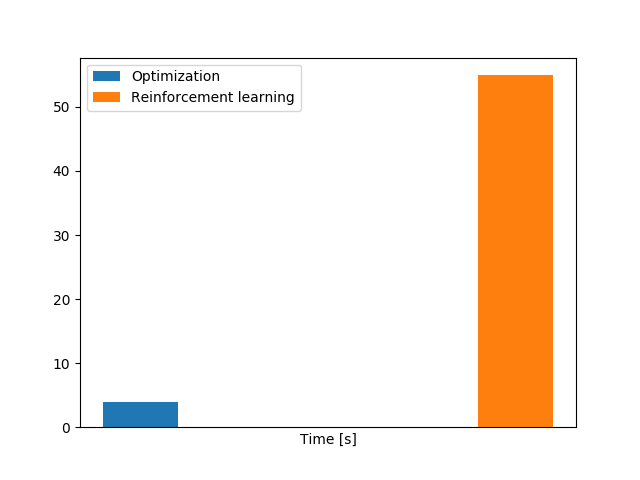
\includegraphics[scale=0.5]{img/time}
\caption{Comparion of the total time of the two methods.}
\label{fig:time}
\end{figure}

As we can see on the figure, the RL method takes more than 10 times the time of the optimization method.
However, note that the assumptions of the multi-time-steps optimization program are quite strict.
If we would have added the flexible load and the uncertainty, the modelisation as an optimization program would have been more complicated and the time would have increased. 

\subsection{Results}
% section results (end)
